\documentclass[10pt]{beamer}

\usepackage{textpos}
\usepackage{tikz,calc}

\usepackage[english]{babel}
\usepackage{multicol}
\usepackage{float}
\usepackage{multirow}
\restylefloat{table}
\usepackage{graphics}
\usepackage{multimedia}
\usepackage{times}
\usepackage{graphicx}
\usepackage{epstopdf}
\usepackage{epsfig}
\usepackage{epsf}
\usepackage{rotating}
\usepackage[bf,SL,BF]{subfigure}
\usepackage{verbatim}
\usepackage{amsmath}
\usepackage{paralist}
\usepackage{amsfonts,amsthm,amssymb}
\usepackage{colordvi}
\usepackage{color}
\usepackage{setspace}
\usepackage{latexsym,wasysym,mathrsfs}

\DeclareGraphicsExtensions{.pdf,.png,.jpg,.eps,.ps,.jpeg}

\usetheme{Copenhagen}

%% position the logo
%\addtobeamertemplate{frametitle}{}{%
%\begin{textblock*}{100mm}(\textwidth,-0.85cm)
%\includegraphics[height=0.8cm,width=0.8cm,keepaspectratio]{OSU_vertical_2C_O_over_B.png}
%\end{textblock*}}

% ***** New commands for mathematics *****
\newcommand{\bes}{\begin{equation*}}
\newcommand{\ees}{\end{equation*}}
\newcommand{\beq}{\begin{equation}}
\newcommand{\eeq}{\end{equation}}
\newcommand{\barr}{\begin{array}}
\newcommand{\earr}{\end{array}}
\newcommand{\Pb}{\mathbb P}
\newcommand{\Prm}{\mathrm{Pr}}
\newcommand{\E}{\mathbb E}
\newcommand{\R}{\mathbb R}
\newcommand{\Q}{\mathbb Q}
\newcommand{\N}{\mathbb N}
\newcommand{\Z}{\mathbb Z}
\newcommand{\C}{\mathbb C}
\newcommand{\la}{\langle}
\newcommand{\ra}{\rangle}
\newcommand{\mA}{\bf A}
\newcommand{\mB}{\bf B}
\newcommand{\mC}{\bf C}
\newcommand{\ve}{\varepsilon}
\newcommand{\dl}{\delta}
\newcommand{\rar}{\rightarrow}
\newcommand{\lra}{\longrightarrow}
\newcommand{\Rar}{\Rightarrow}
\newcommand{\Lra}{\Longrightarrow}
\newcommand{\oo}{\infty}
\newcommand{\si}{\sigma}
\newcommand{\prt}{\partial}
\newcommand{\ka}{\kappa}
\newcommand{\J}{\mathcal J}
\newcommand{\mO}{\mathcal O}
\newcommand{\D}{\mathcal D}
\newcommand{\x}{\sf x}
\newcommand{\z}{\sf z}
\newcommand{\risk}{\mathcal{R}}
\newcommand{\Hyp}{\mathscr{H}}
\newcommand{\Ls}{\mathscr{L}^2}
\newcommand{\im}{{\tt i}}
\newcommand{\epty}{\bigcirc\hspace{-2.5mm}\big\slash}
\newcommand{\diff}[2]{\frac{\mathrm {#1}}{\mathrm{#1}#2}}
\newcommand{\rl}{\mathrm{l}}
\newcommand{\rh}{\mathrm{h}}
\newcommand{\diag}{\operatorname{diag}}
% ***** Commands for theorems *****
\theoremstyle{plain}
\newtheorem*{lma}{Lemma}
\newtheorem*{thm}{Theorem}
\newtheorem{theorema}{Theorem}[section]
\newtheorem{lema}[theorem]{Lemma}
\newtheorem{cor}[theorem]{Corollary}
\newtheorem{prop}[theorem]{Proposition}
\theoremstyle{definition}
\newtheorem*{ack}{Acknowledgments}
\newtheorem{examp}[theorem]{Example}
\newtheorem{exercise}[theorem]{Exercise}
\newtheorem{defn}[theorem]{Definition}
\newtheorem{defs}{Definition}
\theoremstyle{remark}
\newtheorem{remark}[theorem]{Remark}
\newtheorem{convention}[theorem]{Convention}
\newtheorem{statement}[theorem]{Statement}
\newtheorem{facts}[theorem]{Fact}
\newtheorem{axiom}[theorem]{Axiom}

\usepackage{pgf,tikz}
\usepackage{mathrsfs}
\usetikzlibrary{arrows}
\usetikzlibrary{matrix}
%NEW TIKZ COMMANDS
%\usepackage{verbatim}
%\usepackage[active,tightpage]{preview}
%\PreviewEnvironment{tikzpicture}
%\setlength{\PreviewBorder}{10pt}%
\usetikzlibrary{calc}
\usepackage{amssymb}

\usepackage[weather]{ifsym}

%Empty header
\makeatletter
    \newenvironment{withoutheadline}{
        \setbeamertemplate{headline}[default]
        \def\beamer@entrycode{\vspace*{-\headheight}}
    }{}
\makeatother

\setbeamertemplate{theorems}[numbered]

% Presentation parameters
\title[FMDV in African Buffalo]{FMDV in African Buffalo\\Influence of immunity in the spread 
of wildlife diseases}
\author[Ricardo Reyes]{Ricardo No\'e Gerardo Reyes Grimaldo}
\institute[OSU]{Oregon State University\\ 
\includegraphics[height=1.cm,width=3.cm,keepaspectratio]{OSU_horizontal_1C_B}}
\date{\today}

%\beamertemplatenavigationsymbolsempty % to get rid of nav symbols

\begin{document}
\begin{withoutheadline}
\begin{frame}
\titlepage
\end{frame}
\end{withoutheadline}

%\begin{frame}
%\tableofcontents
%\end{frame}

\section{Problem}
%%%%%%%%%%%%%%%%%%%%%%%%%%%%%%%%%%%%%%%%%%%%%%%%%%%%%%%%%%%%%%%%%%%%%%%%
\subsection{Antibody levels of different serotypes}

\begin{frame}{Foot and Mouth Disease (FMD)}
\begin{itemize}
\item Antibody level dynamics behave like a random walk given by a Markov Process
\bes
P(t\mid \pmb{\theta})=\left(\barr{cc}P_\rl(t\mid t_0=0)&P_\rh(t\mid t_0=0)\\
P_\rl(t\mid t_0=1)&P_\rh(t\mid t_0=1)\earr\right)
\ees
\item The transition probabilities can be described through
\bes
\diff{d}{t}P_\rh(t)=\lambda_\rl(t)-(\lambda_\rl(t)+\lambda_\rh(t))P_\rh(t)=\eta(t)-\gamma(t)
P_\rh(t)
\ees
\item Whenever $\lambda_\rl(t)$ and $\lambda_\rh(t)$ are determined integrable functions, the solution is given by 
\bes
P_\rh(t)=\left(\int_{t_0}^{t}\exp\left\{\int_{t_0}^{s}\gamma(\tau)d\tau\right\}\eta(s)ds-
P_\rh(t_0)\right)\exp\left\{-\int_{t_0}^{t}\gamma(s)ds\right\}
\ees
\end{itemize}
\end{frame}


%%%%%%%%%%%%%%%%%%%%%%%%%%%%%%%%%%%%%%%%%%%%%%%%%%%%%%%%%%%%%%%%%%%%%%%
\subsection{Statistical Analysis}

\begin{frame}{Maximum Likelihood Estimators and two proposed models}
We compare the following two models:
\begin{center}\begin{tabular}{c||cc} 
Model&$\lambda_\rl(t)$&$\lambda_\rh(t)$\\\hline\hline
Model 1&$a$&$b$\\
Model 2&$\displaystyle\left(\frac{\alpha-\beta}{t_{end}-t_{start}}\right)t+\left(
\frac{\alpha-\beta}{t_{end}-t_{start}}t_{start}+\alpha\right)=
ct+d$&$e$\end{tabular}\end{center}
Whenever $\alpha=\beta$ in Model 2, it reduces to Model 1; by using the Maximum Likelihood 
Estimator (MLE) and design the following hypothesis test
\bes
H_0:\quad\alpha=\beta\qquad\mbox{v.s.}\qquad H_1:\alpha\neq\beta
\ees
we can decide which model fits better our experimental data
\end{frame}

\section{Workflow}
%%%%%%%%%%%%%%%%%%%%%%%%%%%%%%%%%%%%%%%%%%%%%%%%%%%%%%%%%%%%%%%%%%%%%%%%
\subsection{Adaptation of the workflow}
\begin{frame}{Proposed Workflow and final workflow}
\begin{center}
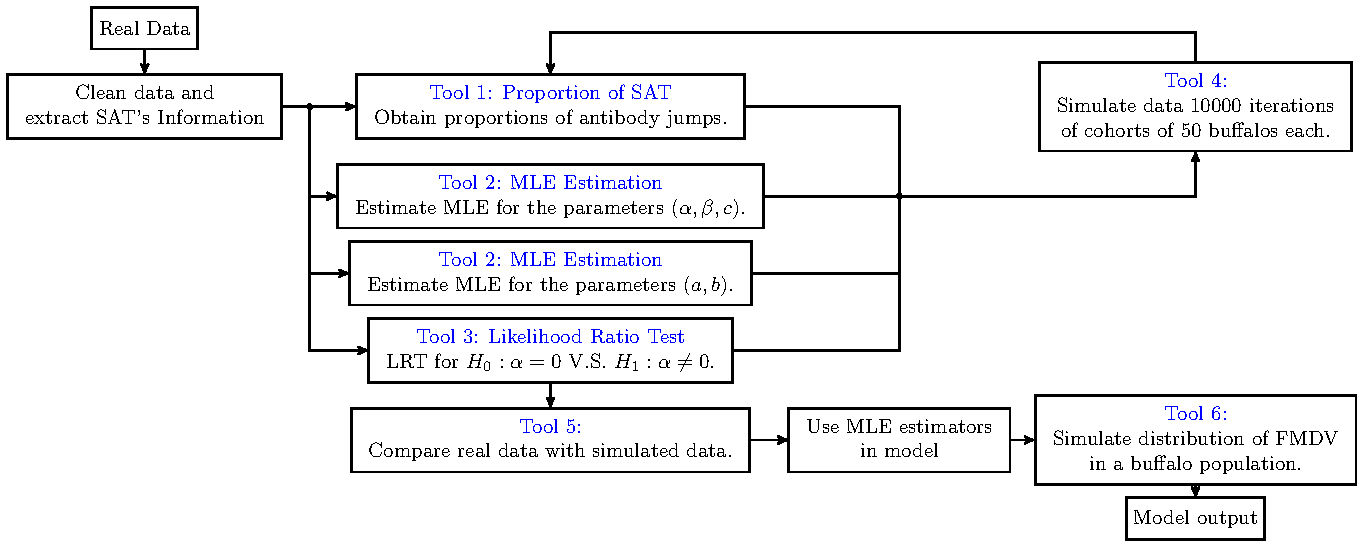
\includegraphics[height=0.3\textheight,width=0.8\textwidth]{Workflow_diagram.pdf}
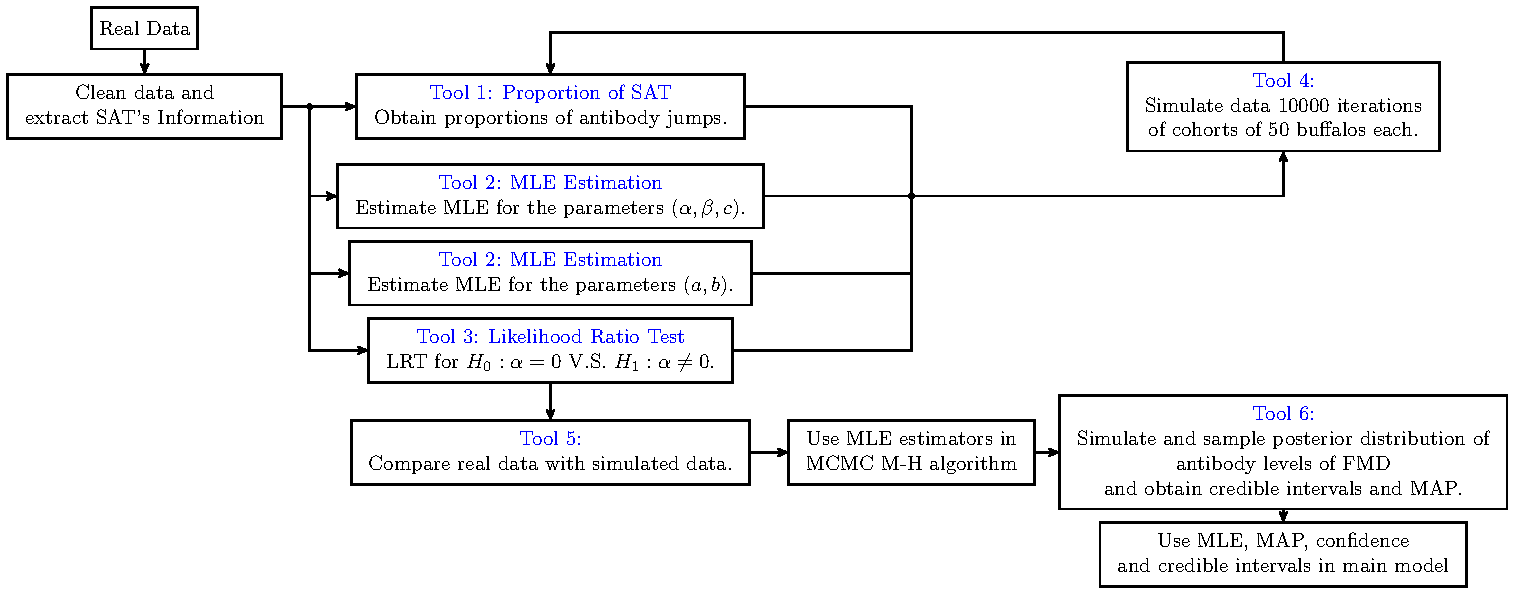
\includegraphics[height=0.3\textheight,width=0.8\textwidth]{Workflow_diagram2.pdf}
\end{center}
For further information see {\color[rgb]{0,0,1} github.com/ricardoreyesgrimaldo/FMDV-immunity}
\end{frame}

\section{Bayesian Results}
%%%%%%%%%%%%%%%%%%%%%%%%%%%%%%%%%%%%%%%%%%%%%%%%%%%%%%%%%%%%%%%%%%%%%%%%
\begin{frame}{Frequentist and Bayesian results for SAT1}
\begin{center}
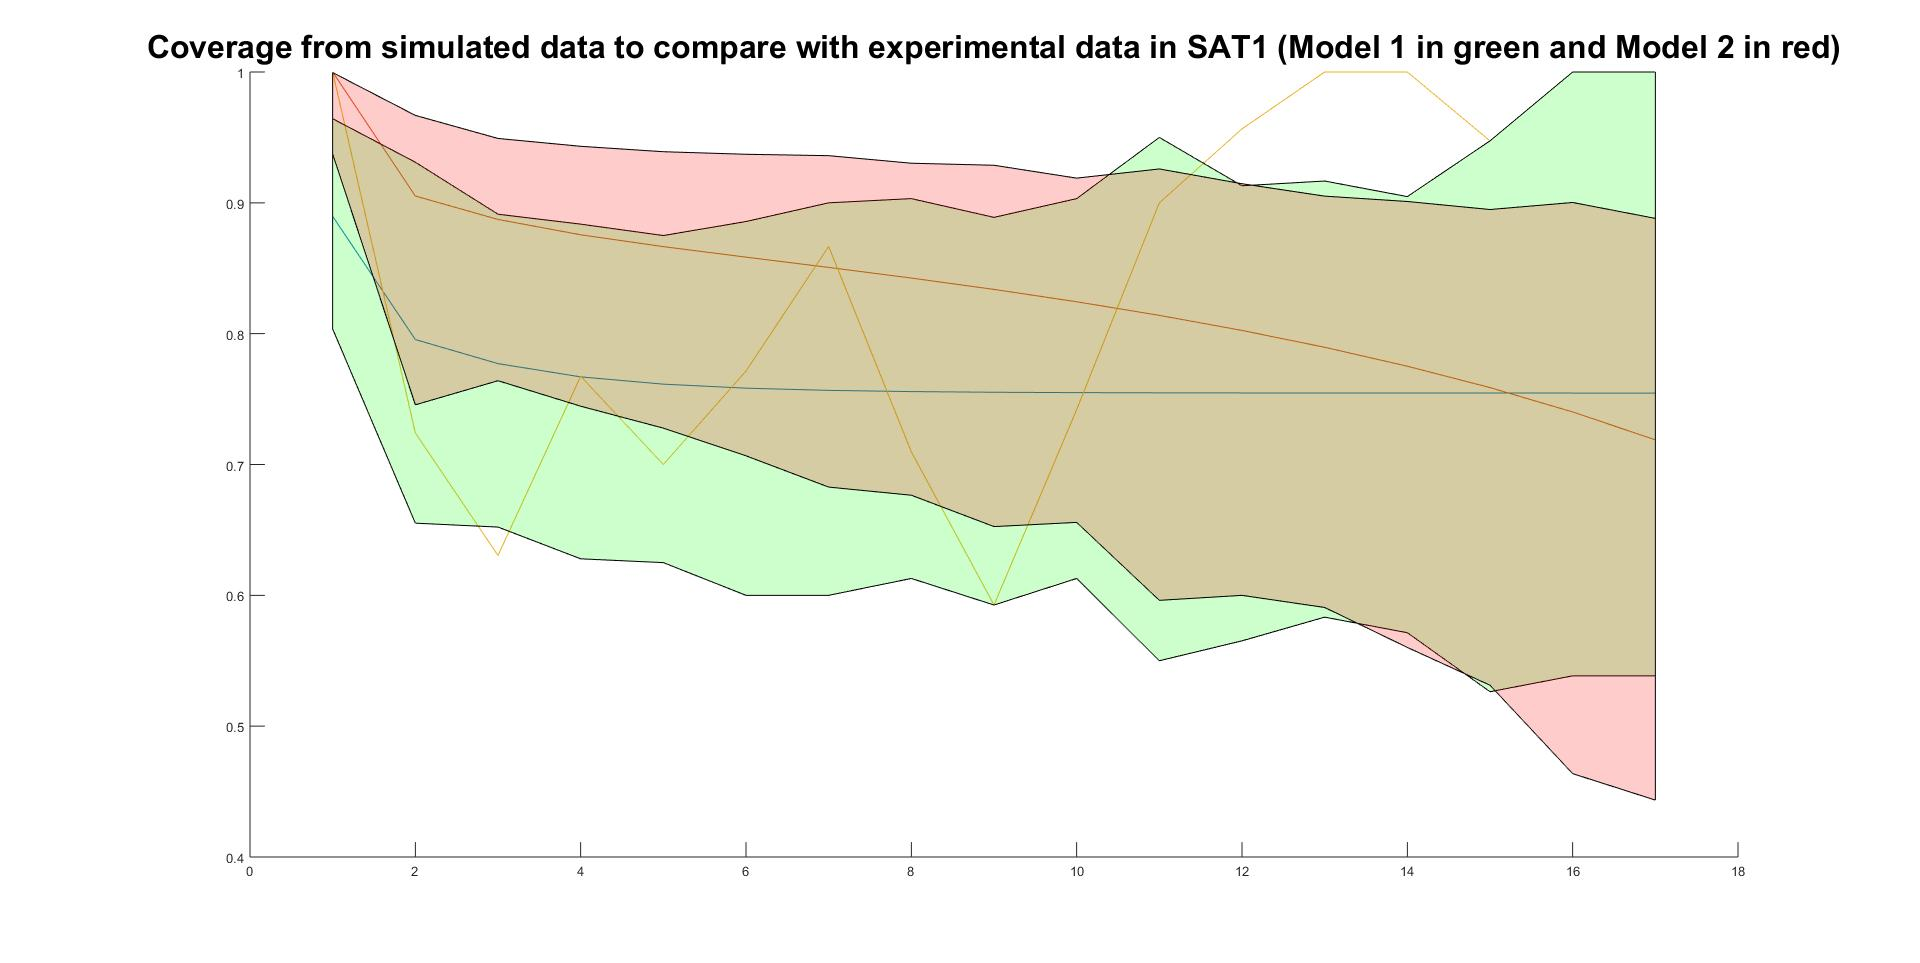
\includegraphics[height=0.4\textheight,width=0.45\textwidth]{fig11.jpg}
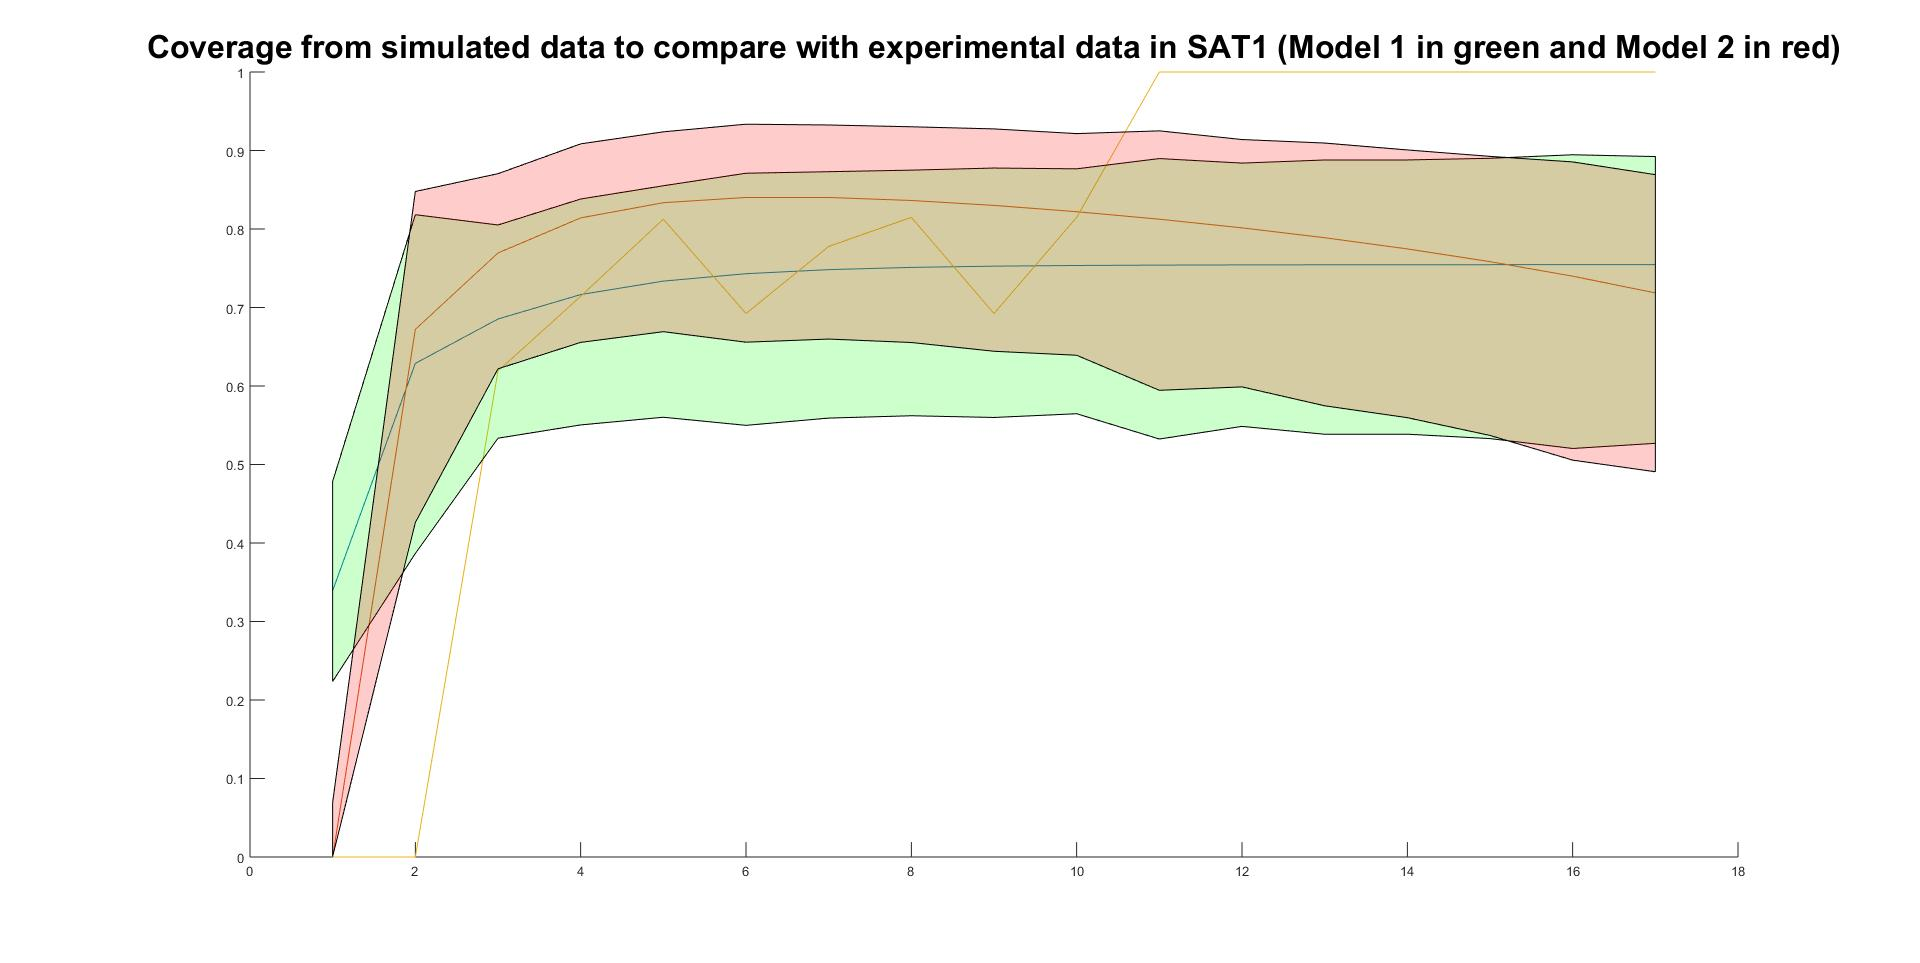
\includegraphics[height=0.4\textheight,width=0.45\textwidth]{fig14.jpg}
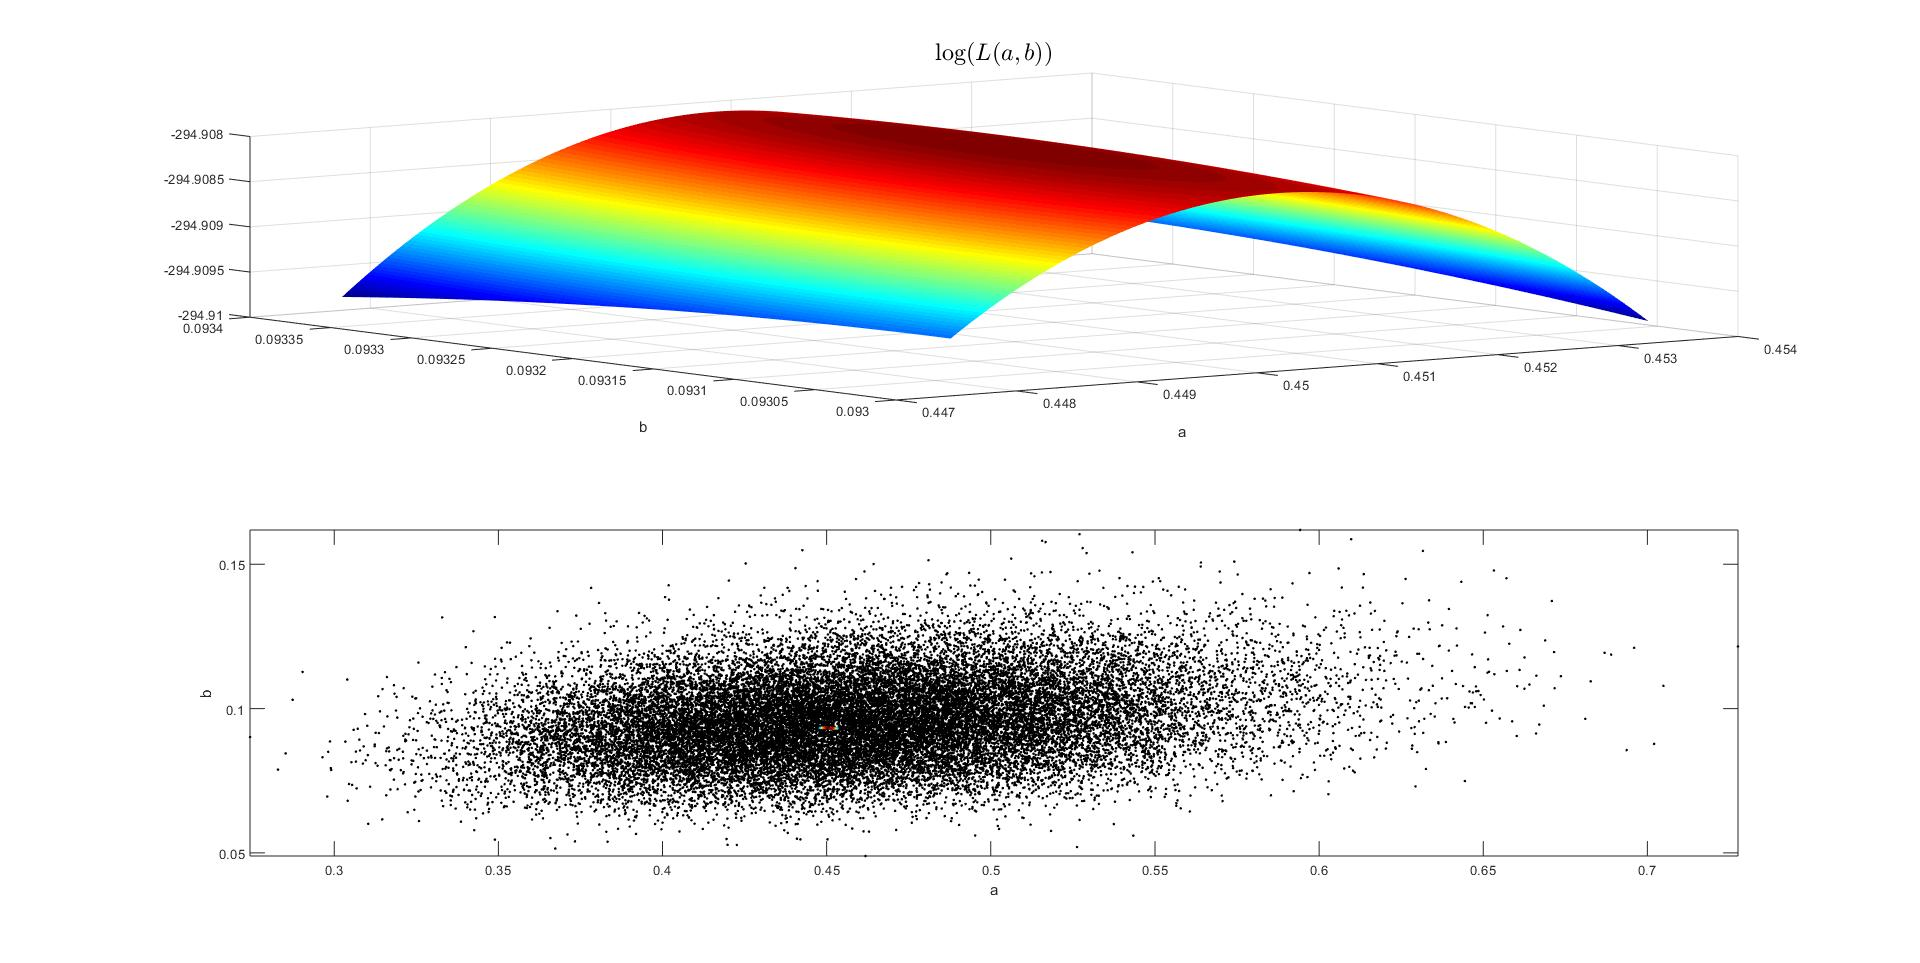
\includegraphics[height=0.4\textheight,width=0.45\textwidth]{mcmchcfig2.jpg}
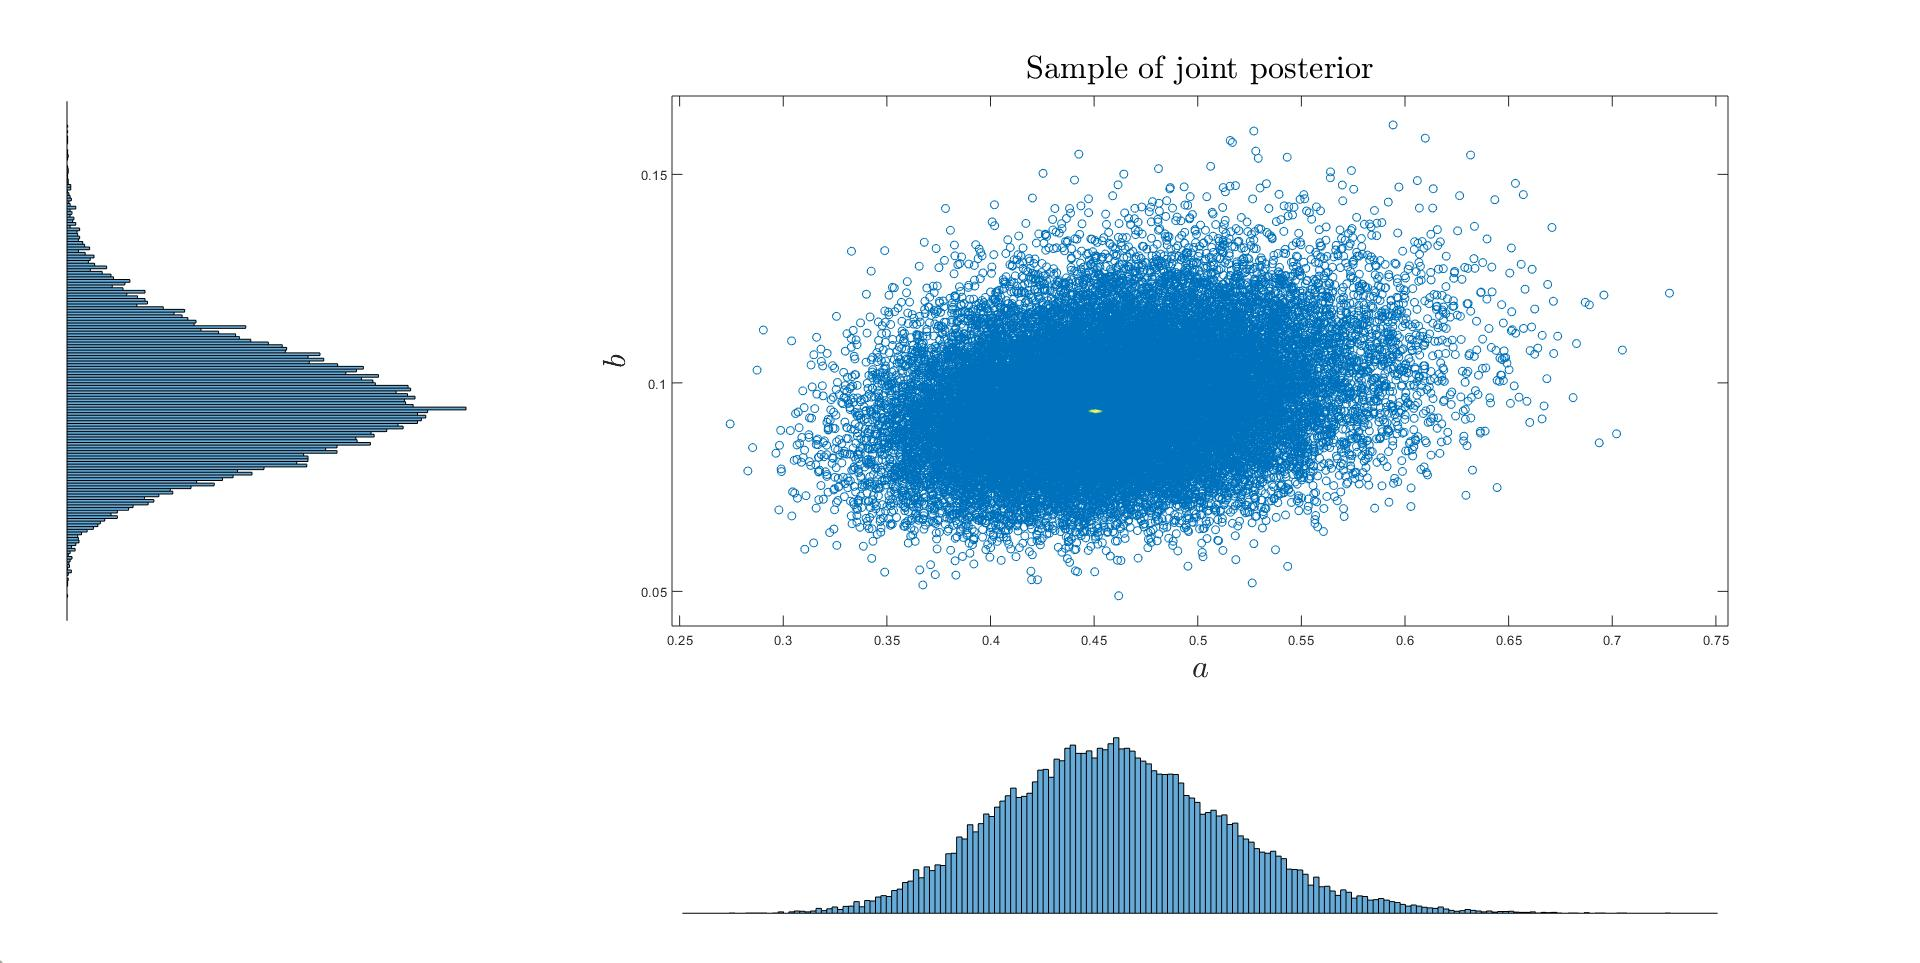
\includegraphics[height=0.4\textheight,width=0.45\textwidth]{mcmchcfig4.jpg}
\end{center}
\end{frame}
\end{document}